
\section{Solr}

\subsection{Installation}

Der empfohlene Installationsweg für Xapian führt über das Paketquelle (PPA) der Entwickler. Nachdem dieses eingefügt wurde, kann Xapian entweder in einer C++ oder Python Variante installiert werden. Damit Xapian auch mit PHP anzusprechen ist, ist es allerdings notwendig den PHP-Connector aus Lizenzgründen selbst zu bauen. Dabei muss vorher der ein Eintrag, der ausweist, dass aus dieser Quelle auch Source-Code geladen werden kann, in der Paketquellen hinzugefügt werden. Nachdem nun der PHP-Klient gebaut worden ist, kann dieser nun normal installiert werden.
Allerdings ist der Server bisher nur Lokal ansprechbar, um dies zu ändern, muss ein TCP-Server für Xapian gestartet werden. Um diesen zu Nutzen ist es vonnöten ein weiteres Paket aus der PPA zu installieren. Damit nun der Server gestartet werden kann, muss zuerst ein Index, der bei Xapian Database genannt wird, gebaut werden. Dazu mehr in dem Teil \ref{xap:index}. Danach kann der Server auf einen beliebigen Port gestartet werden.

\subsection{Indexierung}
\label{xap:index}

Durch die fehlende Dokumentation zur Indexierung von MySQL-Datenbanken, habe ich zuerst einmal ein gegeben Beispiel zur Indexierung von eine CSV Datei durchgearbeitet. Dabei ist mir aufgefallen, dass zur Indexierung ein Parser für MySQL-Daten zu Xapian komplett selbst geschrieben werden muss. Soll nun also eine Datenbank indexiert werden, muss die Datenbank selbst durchsucht und die einzelnen Felder an Xapian weitergegeben werden.  

Um nun die Daten von der Datenbank in Xapian zu indeixeren, muss nun eine Sprache in der es möglich ist eine Datenbankverbindung aufzubauen benutzt werden. Ich hab mich dabei für PHP entschieden. Die Indexierung läuft dabei folgendermaßen ab. !!!!

Als nun das PHP-Script auf den Server gestartet wurde, mussten noch einen Warnungen und Fehler behoben werden. Dazu wurde die php.ini angepasst. 

$PHP WARNING -> PHP Warning:  dl(): Dynamically loaded extensions aren't enabled in /usr/share/php/xapian.php on line 22$


\subsection{Oberfläche}

Xapian besitzt keine Oberfläche zur Verwaltung. Allerdings kann sich ein Such-Frontend installiert werden, welches allerdings hier nicht geprüft wurde, da beim Dietrich sowieso ein eigenes Frontend gebaut werden musste.

\subsection{Dokumentation}

Bei dem letzten Versionsupgrade wurde die Dokumentation von Xapian komplett umgeschrieben. Diese neue Dokumentation hat bisher noch viele Lücken und besitzt auch Todo-Boxen \ref{img:xapianDoku}.
Zu der Installation von dem TCP-Server war nichts in der neuen Dokumentation zu finden. Durch Googlen, wie der Server extern ansprechbar gemacht werden kann, bin ich zufällig auf eine Seite der Dokumentation gestoßen, welche einen Befehl zum Starten vermerkt hatte. Nachdem dieser Befehl ausgeführt wurde, wurde gemeldet, dass für diesen Befehl ein weiteres Paket installiert werden musste. Dieses Paket wurde in der Dokumentation nicht genannt. 

Generell bietet die Dokumentation bisher nur einen sehr grundlegenden Einblick in das System und beleuchtet keine genauen Themen, wie das Indexieren von MySQL-Datenbanken. Positiv anzumerken ist allerdings, dass Xapian ein Beispiel zu Indexierung von Daten mit Code bereitstellt. Allerdings ist dieses nur in Python verfügbar.

\begin{figure}
	\centering
	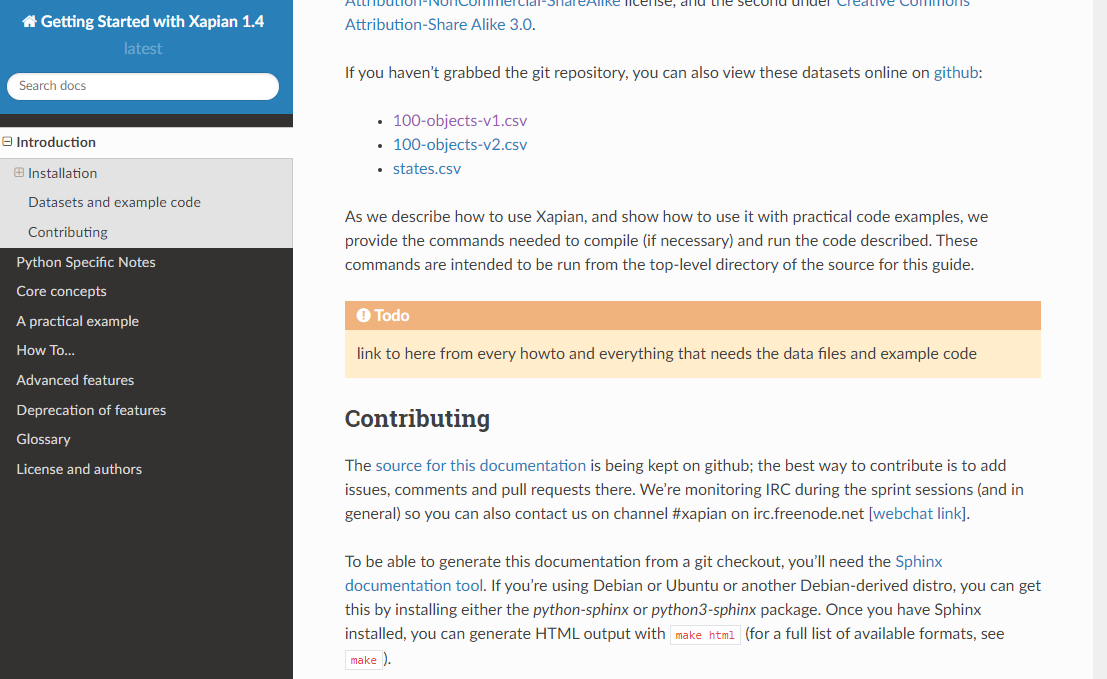
\includegraphics[width=1\linewidth]{images/xapian_doku.png}
	\caption{Screenshot von der Xapian-Dokumentation}
	\label{img:xapianDoku}
\end{figure}


\subsection{Absetzen einer Anfrage und Integration in PHP}

